%--------------------------------------------------------------------------------------------------
% 
\chapter{Autonomous Data Cleaning on a Stream}
\label{ch:data-cleaning}
%--------------------------------------------------------------------------------------------------

\highlight{COMMENT}
V tem primeru mora biti iz uvoda jasno razviden opis znanstvene metode ter prispevka kandidata k posamezni objavi, pri kateri je več avtorjev. V diskusiji kandidat smiselno povzame vse rezultate svoje disertacije.
\highlight{ENDCOMMENT}

TODO

\begin{list}{}
{\leftmargin=2.5em \itemindent=-2.5em}
    \item K. Kenda and D. Mladenić, “Autonomous sensor data cleaning in stream mining setting,” \textit{Business Systems Research Journal}, vol. 9, no. 2, pp. 69–79, 2018.
\end{list}


\begin{quote}
    \textit{Klemen Kenda contributed to the conceptualization, methodology, software development, evaluation and visualization. He also lead writing of the paper.}
\end{quote}

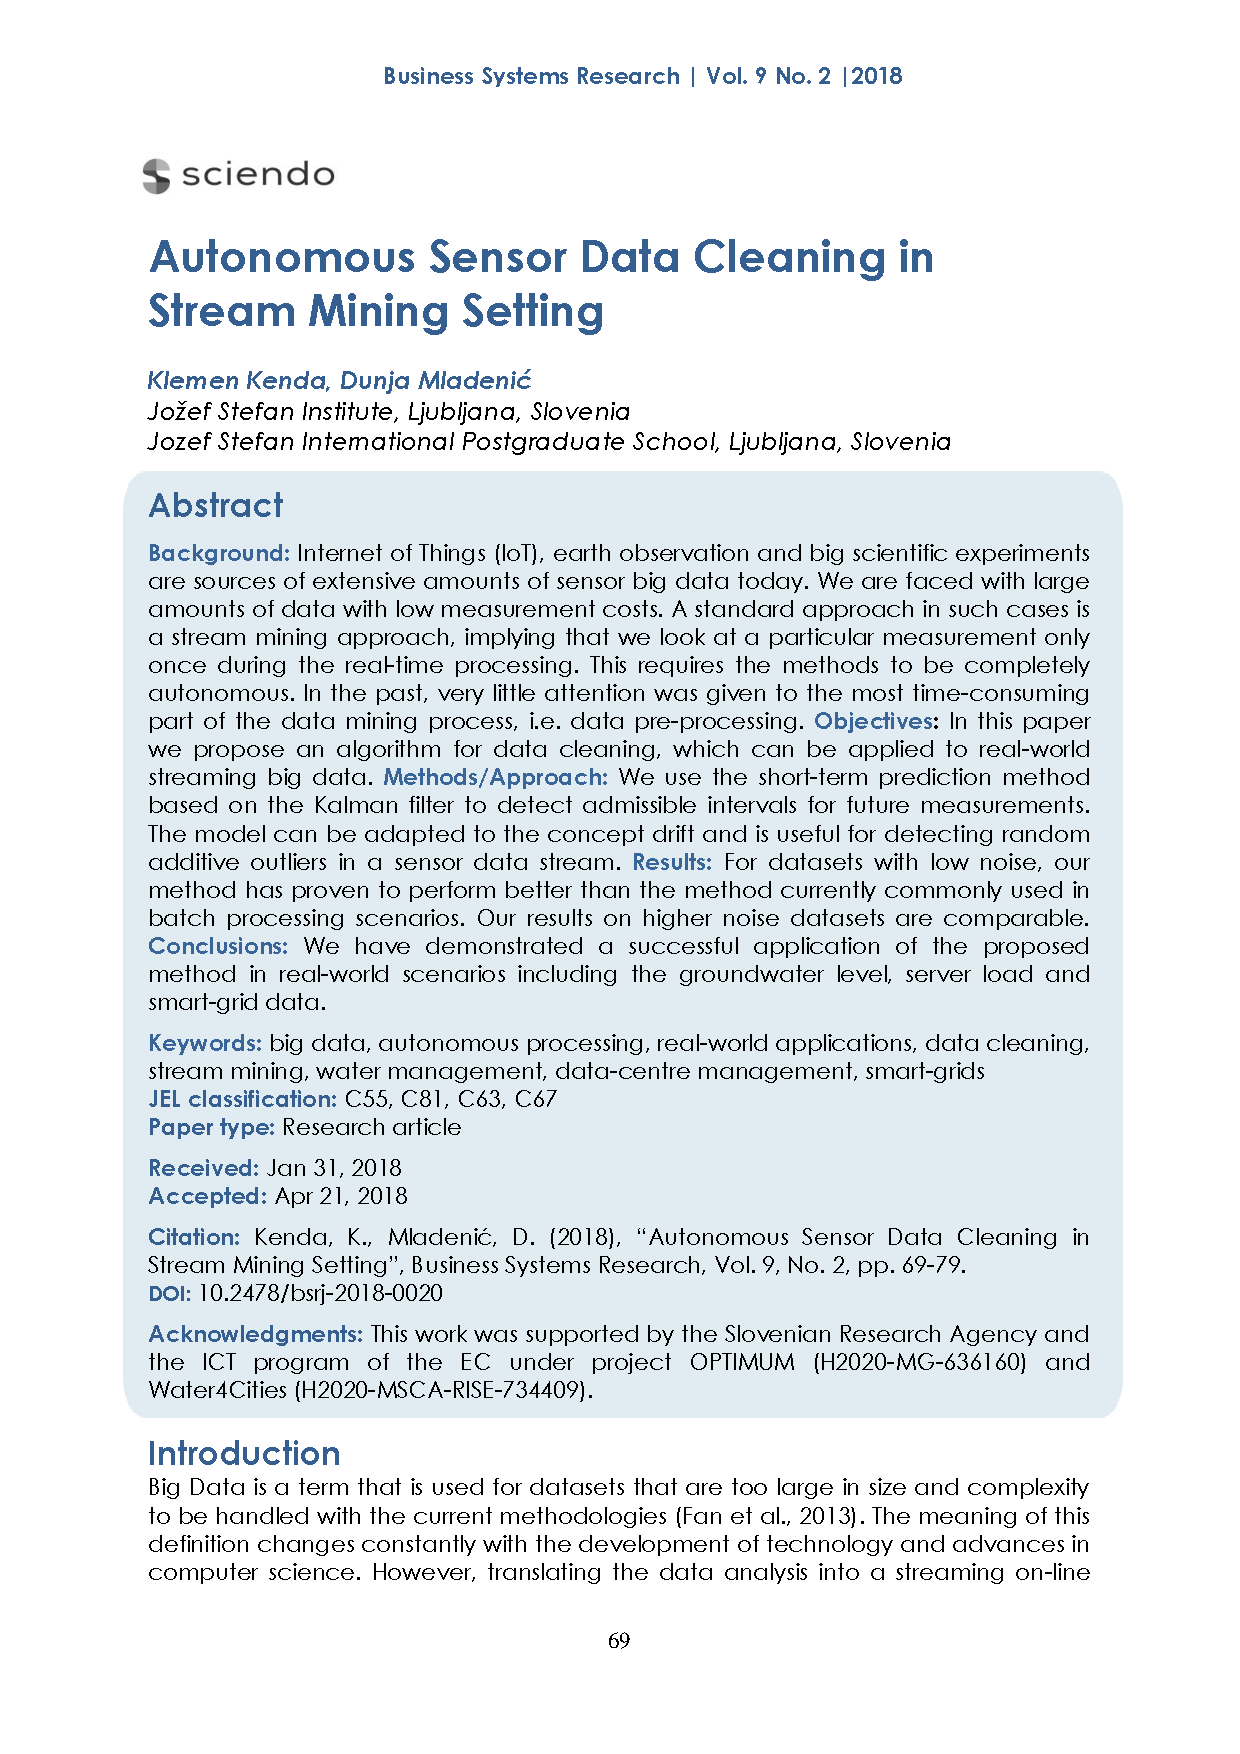
\includepdf[pages=-]{papers/data_cleaning.pdf}